\documentclass[12pt,a4paper]{report}
\usepackage[utf8]{inputenc}
\usepackage[a4paper,top=1in,bottom=1in,left=1in,right=1in]{geometry}
\usepackage{graphicx}
\usepackage{booktabs}
\usepackage{fancyhdr}
\usepackage{hyperref}
\usepackage{listings}
\usepackage{xcolor}
\usepackage{setspace}
\usepackage{tikz}

% Page border matching SKIT standard template (10mm from edges)
\usepackage{eso-pic}
\AddToShipoutPictureBG{%
  \begin{tikzpicture}[remember picture,overlay]
    \draw[line width=1pt] 
      ([shift={(10mm,-10mm)}]current page.north west) 
      rectangle 
      ([shift={(-10mm,10mm)}]current page.south east);
  \end{tikzpicture}%
}

\hypersetup{
    colorlinks=true,
    linkcolor=black,
    urlcolor=blue,
    citecolor=black
}

\definecolor{codegray}{rgb}{0.5,0.5,0.5}
\definecolor{codepurple}{rgb}{0.58,0,0.82}
\definecolor{backcolour}{rgb}{0.97,0.97,0.97}

\lstdefinestyle{mystyle}{
    backgroundcolor=\color{backcolour},   
    commentstyle=\color{codegray},
    keywordstyle=\color{blue},
    numberstyle=\tiny\color{codegray},
    stringstyle=\color{codepurple},
    basicstyle=\ttfamily\footnotesize,
    breakatwhitespace=false,         
    breaklines=true,                 
    captionpos=b,                    
    keepspaces=true,                 
    numbers=left,                    
    numbersep=5pt,                  
    showspaces=false,                
    showstringspaces=false,
    showtabs=false,                  
    tabsize=2
}
\lstset{style=mystyle}

\onehalfspacing

\begin{document}

% ================= COVER PAGE =================
\begin{titlepage}
\begin{center}
    \vspace*{0.5cm}
    {\huge\textbf{INDUSTRIAL TRAINING REPORT}\par}
    \vspace{0.8cm}
    {\Large\textbf{LAMIWOOD: AN E-COMMERCE PLATFORM FOR\\PREMIUM INTERIOR SURFACES}\par}
    
    \vspace{1.2cm}
    {\normalsize Submitted in partial fulfilment of the\\Requirements for the award of\par}
    \vspace{0.2cm}
    {\large\textbf{Degree of Bachelor of Technology in Computer Science \& Engineering}\par}
    
    \vspace{1.0cm}
    
\includegraphics[width=3.5cm]{assets/page_1_img_1.png}\par
    \vspace{0.6cm}
    
    {\large\textbf{Session: 2026--27}\par}
    \vspace{0.8cm}
    
    \textbf{Submitted By}\par
    \vspace{0.3cm}
    \begin{tabular}{ll}
        Name: & \underline{\textbf{Aditya Swami}} \\
        University Roll No.: & \underline{\textbf{24ESKCS024}} \\
        Semester/Branch: & \underline{\textbf{5th Semester / CSE}}
    \end{tabular}
    
    \vfill
    {\large\textbf{SUBMITTED TO:}\par}
    \vspace{0.2cm}
    {\large\textbf{Department of Computer Science \& Engineering}\par}
    \vspace{0.1cm}
    {\large\textbf{SWAMI KESHVANAND INSTITUTE OF TECHNOLOGY,\\MANAGEMENT \& GRAMOTHAN, JAIPUR}\par}
    \vspace*{0.5cm}
\end{center}
\end{titlepage}

\pagenumbering{roman}

% ================= DECLARATION =================
\chapter*{DECLARATION}
\addcontentsline{toc}{chapter}{Declaration}
I hereby declare that the Industrial Training Report entitled \textbf{``Lamiwood: An E-Commerce Platform for Premium Interior Surfaces''} is an authentic record of my own work as requirements of 6-weeks Industrial Training during the period from 15 May 2026 to 29 June 2026 for the award of degree of B.Tech. (Computer Science \& Engineering), Swami Keshvanand Institute of Technology, Management \& Gramothan, Jaipur, under the guidance of \textbf{Vikash Dhankar} (Faculty Facilitator).

\vspace{2.5cm}
\begin{flushright}
(Signature of Student)\\[0.4cm]
\textbf{Aditya Swami}\\
24ESKCS024
\end{flushright}

\vspace{1.5cm}
\noindent Date:\dotfill\\[0.8cm]
Certified that the above statement made by the student is correct to the best of our knowledge and belief.\\[1.5cm]

\noindent\textbf{Examined by:}\\[1.5cm]

\noindent
\begin{minipage}[t]{0.48\textwidth}
(Signature)\\[0.4cm]
\textbf{Vikash Dhankar}\\
Faculty Facilitator
\end{minipage}
\hfill
\begin{minipage}[t]{0.48\textwidth}
\begin{flushright}
(Signature)\\[0.4cm]
\textbf{Prof.(Dr. Mehul Mahrishi)}\\
Head of Department
\end{flushright}
\end{minipage}

\newpage

% ================= CERTIFICATE =================
\chapter*{CERTIFICATE}
\addcontentsline{toc}{chapter}{Certificate}
\begin{center}
    \vspace*{1cm}
    
\includegraphics[width=0.95\textwidth]{assets/aditya_swami_certificate.png}
\end{center}

\newpage

% ================= ACKNOWLEDGEMENT =================
\chapter*{ACKNOWLEDGEMENT}
\addcontentsline{toc}{chapter}{Acknowledgement}
First and foremost, I wish to express my sincere thanks and gratitude to my esteemed Mentor \textbf{``Mr. Aditya Pareek''} (Founder \& CEO, Linkstatic Techno) who has contributed so much for successful completion of my Industrial Training by his thoughtful reviews, technical expertise, and valuable guidance.

Next I would like to tender my sincere thanks to \textbf{``Prof.(Dr. Mehul Mahrishi)''} (Head of Computer Science \& Engineering) for his co-operation, academic leadership, and continuous encouragement throughout this tenure.

I am also thankful to \textbf{Mr. Vikram Khandelwal}, Coordinator (III Year In-house Internship 2026--27), for his support, administrative cooperation and motivation provided during the internship for constant inspiration, presence and blessings.

Finally, I extend my heartfelt appreciation to the faculty members of the Department of Computer Science \& Engineering and my peers at Swami Keshvanand Institute of Technology, Management \& Gramothan, Jaipur, whose constructive feedback and discussions greatly assisted me during the development and documentation of this project.

\vspace{3cm}
\begin{flushright}
(Signature of Student)\\[0.4cm]
\textbf{Aditya Swami}\\
24ESKCS024
\end{flushright}

\newpage

% ================= ABSTRACT =================
\chapter*{ABSTRACT}
\addcontentsline{toc}{chapter}{Abstract}
The procurement and specification of luxury interior surfaces---including engineered hardwood flooring, architectural acoustic wall panels, outdoor composite decking, and decorative cladding---have traditionally been constrained by cumbersome offline sample distribution and fragmented catalog browsing. This report presents \textbf{Lamiwood}, a modern, production-ready e-commerce web platform engineered during the six-week Industrial Training at Linkstatic Techno in the domain of Full Stack Web and Frontend Engineering.

The platform bridges the gap between digital discovery and architectural precision by delivering a high-performance single-page web application built with \textbf{React 19, TypeScript, Tailwind CSS v4, and Framer Motion}. Lamiwood features a curated product catalog organized across six specialized categories (Flooring, Wall Panels, Decking, Ceiling Panels, Cladding, and Acoustic Panels). To assist homeowners, architects, and interior designers in technical decision-making, the application incorporates custom-engineered interactive tools: an \textbf{Installation Pattern Designer} supporting six distinct floor and wall layouts (Straight, Herringbone, Chevron, Brick Offset, Basket Weave, and Diagonal) with live SVG rendering; an intelligent \textbf{Surface Price \& Wastage Calculator} that accounts for room geometry and layout wastage factors; a real-time \textbf{Side-by-Side Product Comparison Matrix}; and an interactive \textbf{Wood Finish Aging Simulator} illustrating surface patina evolution over a 20-year span.

The architecture adheres to strict component-driven design principles with client-side state persistence. Shopping cart items, technical sample requests, and design wishlists are managed seamlessly via React Context API and synchronized with browser LocalStorage. Client-side routing is handled through React Router 7 with route-level code splitting via \texttt{React.lazy()} and fallback error boundaries. Fluid micro-interactions, luxury staggered text reveals, and scroll-triggered section entrances provide an engaging user experience while maintaining sub-second initial load times and top-tier Google Lighthouse audit ratings.

\vspace{0.8cm}
\noindent\textbf{Keywords:} E-Commerce Platform, Architectural Surfaces, React 19, TypeScript, Tailwind CSS v4, Framer Motion, Pattern Designer, Material Area Calculator, Component-Driven Design.

\newpage

% ================= TABLE OF CONTENTS =================
\tableofcontents
\newpage

\pagenumbering{arabic}

% ================= CHAPTER 1 =================
\chapter{Introduction}

\section{Project Description}
\textbf{Lamiwood} is a premier architectural surfaces and interior design e-commerce web platform engineered to transform how architects, interior designers, commercial developers, and modern homeowners explore, calculate, and procure high-end surfacing solutions. In the architectural materials industry, selecting elements such as engineered European oak flooring, acoustic fluted wall panels, exterior bamboo decking, and decorative charred cladding involves complex spatial, aesthetic, and mathematical evaluations. Traditional digital commerce stores often fail to provide the sensory richness, technical precision, and installation calculators required for high-investment architectural finishes.

The project was developed during a six-week Industrial Training at \textbf{Linkstatic Techno} in the domain of Full Stack Web and Modern Frontend Engineering. Lamiwood addresses industry bottlenecks by providing an interactive digital showroom coupled with precision architectural utilities. Built using \textbf{React 19, TypeScript, Tailwind CSS v4, and Framer Motion}, the platform combines a curated 16-product catalog across 6 core architectural categories with dynamic calculation engines: an interactive \textbf{Installation Pattern Designer}, a \textbf{Room Surface \& Wastage Calculator}, a \textbf{Multi-Product Side-by-Side Comparison Matrix}, and an interactive \textbf{Wood Aging Simulator}. The application tagline, \textit{``Surfaces Crafted for Extraordinary Spaces''}, reflects its core mission: empowering professionals and homeowners to visualize, plan, and specify premium architectural surfaces with absolute confidence.

\section{Project Scope}
The scope of the project encompasses the complete engineering lifecycle of a high-performance, component-driven architectural e-commerce single-page application (SPA), ranging from requirements gathering and design token structuring to state persistence and interactive layout computation:
\begin{itemize}
    \item Architecting a modular, type-safe product schema in TypeScript covering product dimensions, grain finishes, wear-layer thickness, installation click-lock specifications, and certifications.
    \item Developing an immersive, responsive frontend design system adhering to modern luxury interior brand guidelines using Tailwind CSS v4 and Google Fonts typography (Cormorant Garamond and DM Sans).
    \item Implementing multi-faceted client-side catalog filtering and sorting by category, price tier, surface finish, and availability with seamless URL state synchronization.
    \item Engineering mathematical visual tools, including an interactive SVG-driven pattern designer supporting six geometric laying patterns with dynamic room dimensions and wastage percentage algorithms.
    \item Building an end-to-end room area, packaging unit, and budget estimator capable of computing net square footage, buffer margins, and box breakdown for floors, walls, and ceilings.
    \item Providing client-side transactional workflows, including a persistent slide-in Cart Drawer, Technical Sample Request system, and Design Consultation booking modal.
    \item Integrating responsive mobile navigation, scroll-driven header transformations, preloader brand entrance animations, and full-screen lightbox galleries.
\end{itemize}

\section{Intended Users}
Lamiwood is designed to cater to both professional trade specifiers and direct retail clients:
\begin{itemize}
    \item \textbf{Architects and Interior Designers:} Specifiers requiring exact technical dimensions, fire-resistance ratings, acoustic coefficients, installation patterns, and physical sample deliveries for client pitch decks.
    \item \textbf{Luxury Homeowners:} Individuals undertaking residential renovations who seek visual clarity regarding plank layouts, finish durability, and estimated project expenditures without navigating complex sales representatives.
    \item \textbf{General Contractors \& Flooring Installers:} Construction professionals requiring accurate square-foot material breakdowns, packaging unit calculations, and recommended buffer wastage factors.
    \item \textbf{Frontend Developers \& Engineering Students:} Software practitioners seeking reference implementations of cutting-edge React 19 architecture, complex SVG algorithmic rendering, and zero-runtime CSS workflows.
\end{itemize}

\section{Project Features}
The core features implemented in the Lamiwood application are outlined below:
\begin{itemize}
    \item \textbf{Curated Architectural Catalog:} Comprehensive display of 16 artisan products across 6 categories (Flooring, Wall Panels, Decking, Ceiling Panels, Cladding, and Acoustic Panels) with badges, high-resolution imagery, and pricing.
    \item \textbf{Multi-Attribute Filtering \& Sorting:} Real-time filtering by category checkboxes, price range brackets, and sorting options (Price Low-to-High, High-to-Low, Alphabetical, and New Arrivals).
    \item \textbf{Interactive Pattern Designer:} Mathematical laying engine allowing users to toggle between Straight, Herringbone, Chevron, Brick Offset, Basket Weave, and Diagonal layouts while computing real-time tile counts and wastage factors.
    \item \textbf{Surface Price \& Area Calculator:} Four-step interactive estimator that accepts room geometry (width \& length in feet), calculates gross area, recommends material buffer percentage (5\% to 18\%), and outputs exact package box counts and total costs.
    \item \textbf{Product Detail \& Technical Specifications:} Detailed product views featuring multi-image gallery crossfade transitions, technical spec tables (dimensions, finish, warranty, wear layer), and related product recommendations.
    \item \textbf{Side-by-Side Product Comparison:} Multi-select comparison matrix enabling users to evaluate up to three surfaces simultaneously across material composition, thickness, finish, warranty, and price per square foot.
    \item \textbf{Wood Aging Simulator:} Interactive visual slider demonstrating the natural color maturation, UV patina shift, and grain stabilization of hardwood finishes from year 0 to year 20.
    \item \textbf{Persistent Cart \& Sample Request System:} Slide-out Cart Drawer managed via React Context and LocalStorage, supporting sample requests, free shipping thresholds, and order notes.
    \item \textbf{Wishlist \& Favoriting:} One-click bookmarking of desired surfaces with persistent heart indicators and a dedicated Wishlist management page.
    \item \textbf{Consultation \& Callback Modals:} Accessible modal overlays enabling prospective clients to schedule on-site architectural consultations or request instant WhatsApp/telephonic callbacks.
    \item \textbf{Micro-Interactions \& Luxury Motion:} Custom cubic-bezier page transitions, scroll-triggered section reveals, magnetic buttons, and dynamic navbar background blur.
\end{itemize}

% ================= CHAPTER 2 =================
\chapter{Tools \& Technology Used}

\section{Software Model Used}
The project was developed following the \textbf{Iterative and Incremental (Agile) Model}. Given the visual and interactive nature of modern e-commerce applications, dividing development into rapid iterative sprints allowed immediate feedback, continuous usability testing, and incremental feature delivery. The five development iterations were:
\begin{enumerate}
    \item \textbf{Iteration 1 --- Architecture \& Core Design System:} Defining TypeScript interfaces for products and categories, configuring Vite and Tailwind CSS v4, and establishing color tokens and font typography.
    \item \textbf{Iteration 2 --- Component Library \& Catalog Implementation:} Building primitive atomic UI components (Button, Badge, Card, Heading), followed by the Product Grid, Filter Sidebar, and Search Overlay.
    \item \textbf{Iteration 3 --- Interactive Visual Tools:} Developing the algorithmic layout engines for the Pattern Designer, Surface Calculator, Aging Simulator, and Product Comparison matrix.
    \item \textbf{Iteration 4 --- State Management \& Persistence:} Implementing React Context providers for Cart, Wishlist, and QuickView with LocalStorage synchronization.
    \item \textbf{Iteration 5 --- Performance Optimization \& Audit:} Implementing route-based code splitting with React.lazy, optimizing image skeletons, and achieving top Google Lighthouse audit scores.
\end{enumerate}

\section{Technology Stack Used}
The technologies and tools employed in building Lamiwood are summarised in Table \ref{tab:tech_stack}.

\begin{table}[htbp]
\centering
\caption{Technology stack of Lamiwood}
\label{tab:tech_stack}
\begin{tabular}{lll}
\toprule
\textbf{Category} & \textbf{Technology} & \textbf{Purpose} \\
\midrule
UI Framework & React 19 & Component-driven declarative UI architecture [1] \\
Programming Language & TypeScript 6 & End-to-end static type safety and interfaces [5] \\
Build System & Vite 8 & Lightning-fast HMR and Rollup bundling [2] \\
Styling Engine & Tailwind CSS v4 & High-performance utility styling with CSS vars [3] \\
Animation Library & Framer Motion 12 & Spring physics, layout animations, transitions [4] \\
Routing System & React Router 7 & Declarative client-side routing and URL sync \\
Typography & @fontsource & Self-hosted Cormorant Garamond \& DM Sans fonts \\
State Management & Context API & Shopping cart, sample requests, wishlist state \\
Development Tools & VS Code, Chrome & Code editing, live debugging, ESLint 9 \\
\bottomrule
\end{tabular}
\end{table}

\section{Product User Interfaces}
Lamiwood features a sophisticated, luxury-inspired design language dominated by warm charcoal backgrounds (\texttt{\#1A1A1A}), gold accent highlights (\texttt{\#B8860B}), and clean neutral surfaces. The visual hierarchy combines classical serif headlines with ultra-readable sans-serif metadata.

\subsection{Design System Tokens}
\begin{itemize}
    \item \textbf{Color Tokens:} Primary dark background (\texttt{\#121212}), elevated container cards (\texttt{\#1E1E1E}), gold accent buttons and badges (\texttt{\#B8860B} / \texttt{\#D4A843}), muted text (\texttt{\#A0A0A0}), and crisp white headers (\texttt{\#FFFFFF}).
    \item \textbf{Typography Tokens:} Headings utilize \textit{Cormorant Garamond} for an artisanal aesthetic; body text utilizes \textit{DM Sans} for optimal legibility across desktop and mobile screens.
\end{itemize}

\section{Design and Implementation Constraints}
\begin{itemize}
    \item \textbf{Zero-Latency Client-Side Performance:} All filtering, search matching, and calculation features were architected to execute entirely on the client without blocking network round-trips.
    \item \textbf{Responsive Layout Integrity:} The interface maintains visual elegance from small mobile screens (375px) to ultra-wide 4K architectural monitors (2560px+).
    \item \textbf{Framer Motion Animation Overhead:} Steady 60 frames-per-second performance is maintained via GPU-accelerated CSS transforms rather than CPU-intensive layout repaints.
    \item \textbf{Algorithmic Pattern Generation:} Layout coordinates accurately represent relative plank dimensions while remaining mathematically constrained to room aspect ratios.
    \item \textbf{State Synchronization without Server DB:} Shopping cart items and favorites survive browser refreshes via resilient LocalStorage serialization.
    \item \textbf{Accessibility \& Semantic Standards:} Full compliance with W3C Web Content Accessibility Guidelines (WCAG 2.2).
\end{itemize}

\section{Data Flow and Dataset Structure}
The application architecture is structured around clean unidirectional data flow. Product specifications, categories, and client testimonials are managed as strongly-typed immutable records in the \texttt{src/data/} module. Table \ref{tab:schema} outlines the data schema.

\begin{table}[htbp]
\centering
\caption{Product Data Schema \& Attribute Fields}
\label{tab:schema}
\begin{tabular}{lll}
\toprule
\textbf{Field Name} & \textbf{TypeScript Type} & \textbf{Description \& Usage} \\
\midrule
id, slug & string & Unique identifier and SEO-friendly URL slug \\
name & string & Official surface product name \\
category & CategoryType & Union: flooring, wall-panels, decking, etc. \\
price, unit & number, string & Unit price in INR and unit (``per sq.ft'') \\
specs & ProductSpec[] & Key-value pairs: Material, Dimensions, Finish \\
features & string[] & Bullet list of engineering features \\
images & string[] & Architectural photography array \\
inStock & boolean & Stock availability status \\
\bottomrule
\end{tabular}
\end{table}

\section{Software and System Requirements}
\begin{itemize}
    \item \textbf{Development Environment:} Node.js runtime version 18.0+ with npm v9.0+; Visual Studio Code.
    \item \textbf{Build Engine:} Vite 8.0+ with TypeScript 6.0 compiler.
    \item \textbf{Client Browser:} Google Chrome 110+, Microsoft Edge 110+, Mozilla Firefox 115+, Apple Safari 16+.
    \item \textbf{Hardware Requirements:} Minimum 4 GB RAM (8 GB recommended) with multi-core CPU.
\end{itemize}

% ================= CHAPTER 3 =================
\chapter{Snapshots}

\section{Flow Chart / Proposed Work}
The architecture of the Lamiwood project is structured into two core engineering dimensions: the Build \& Component Pipeline (Figure \ref{fig:flow1}) and the Interactive Client Runtime Workflow (Figure \ref{fig:flow2}).

\begin{figure}[htbp]
\centering
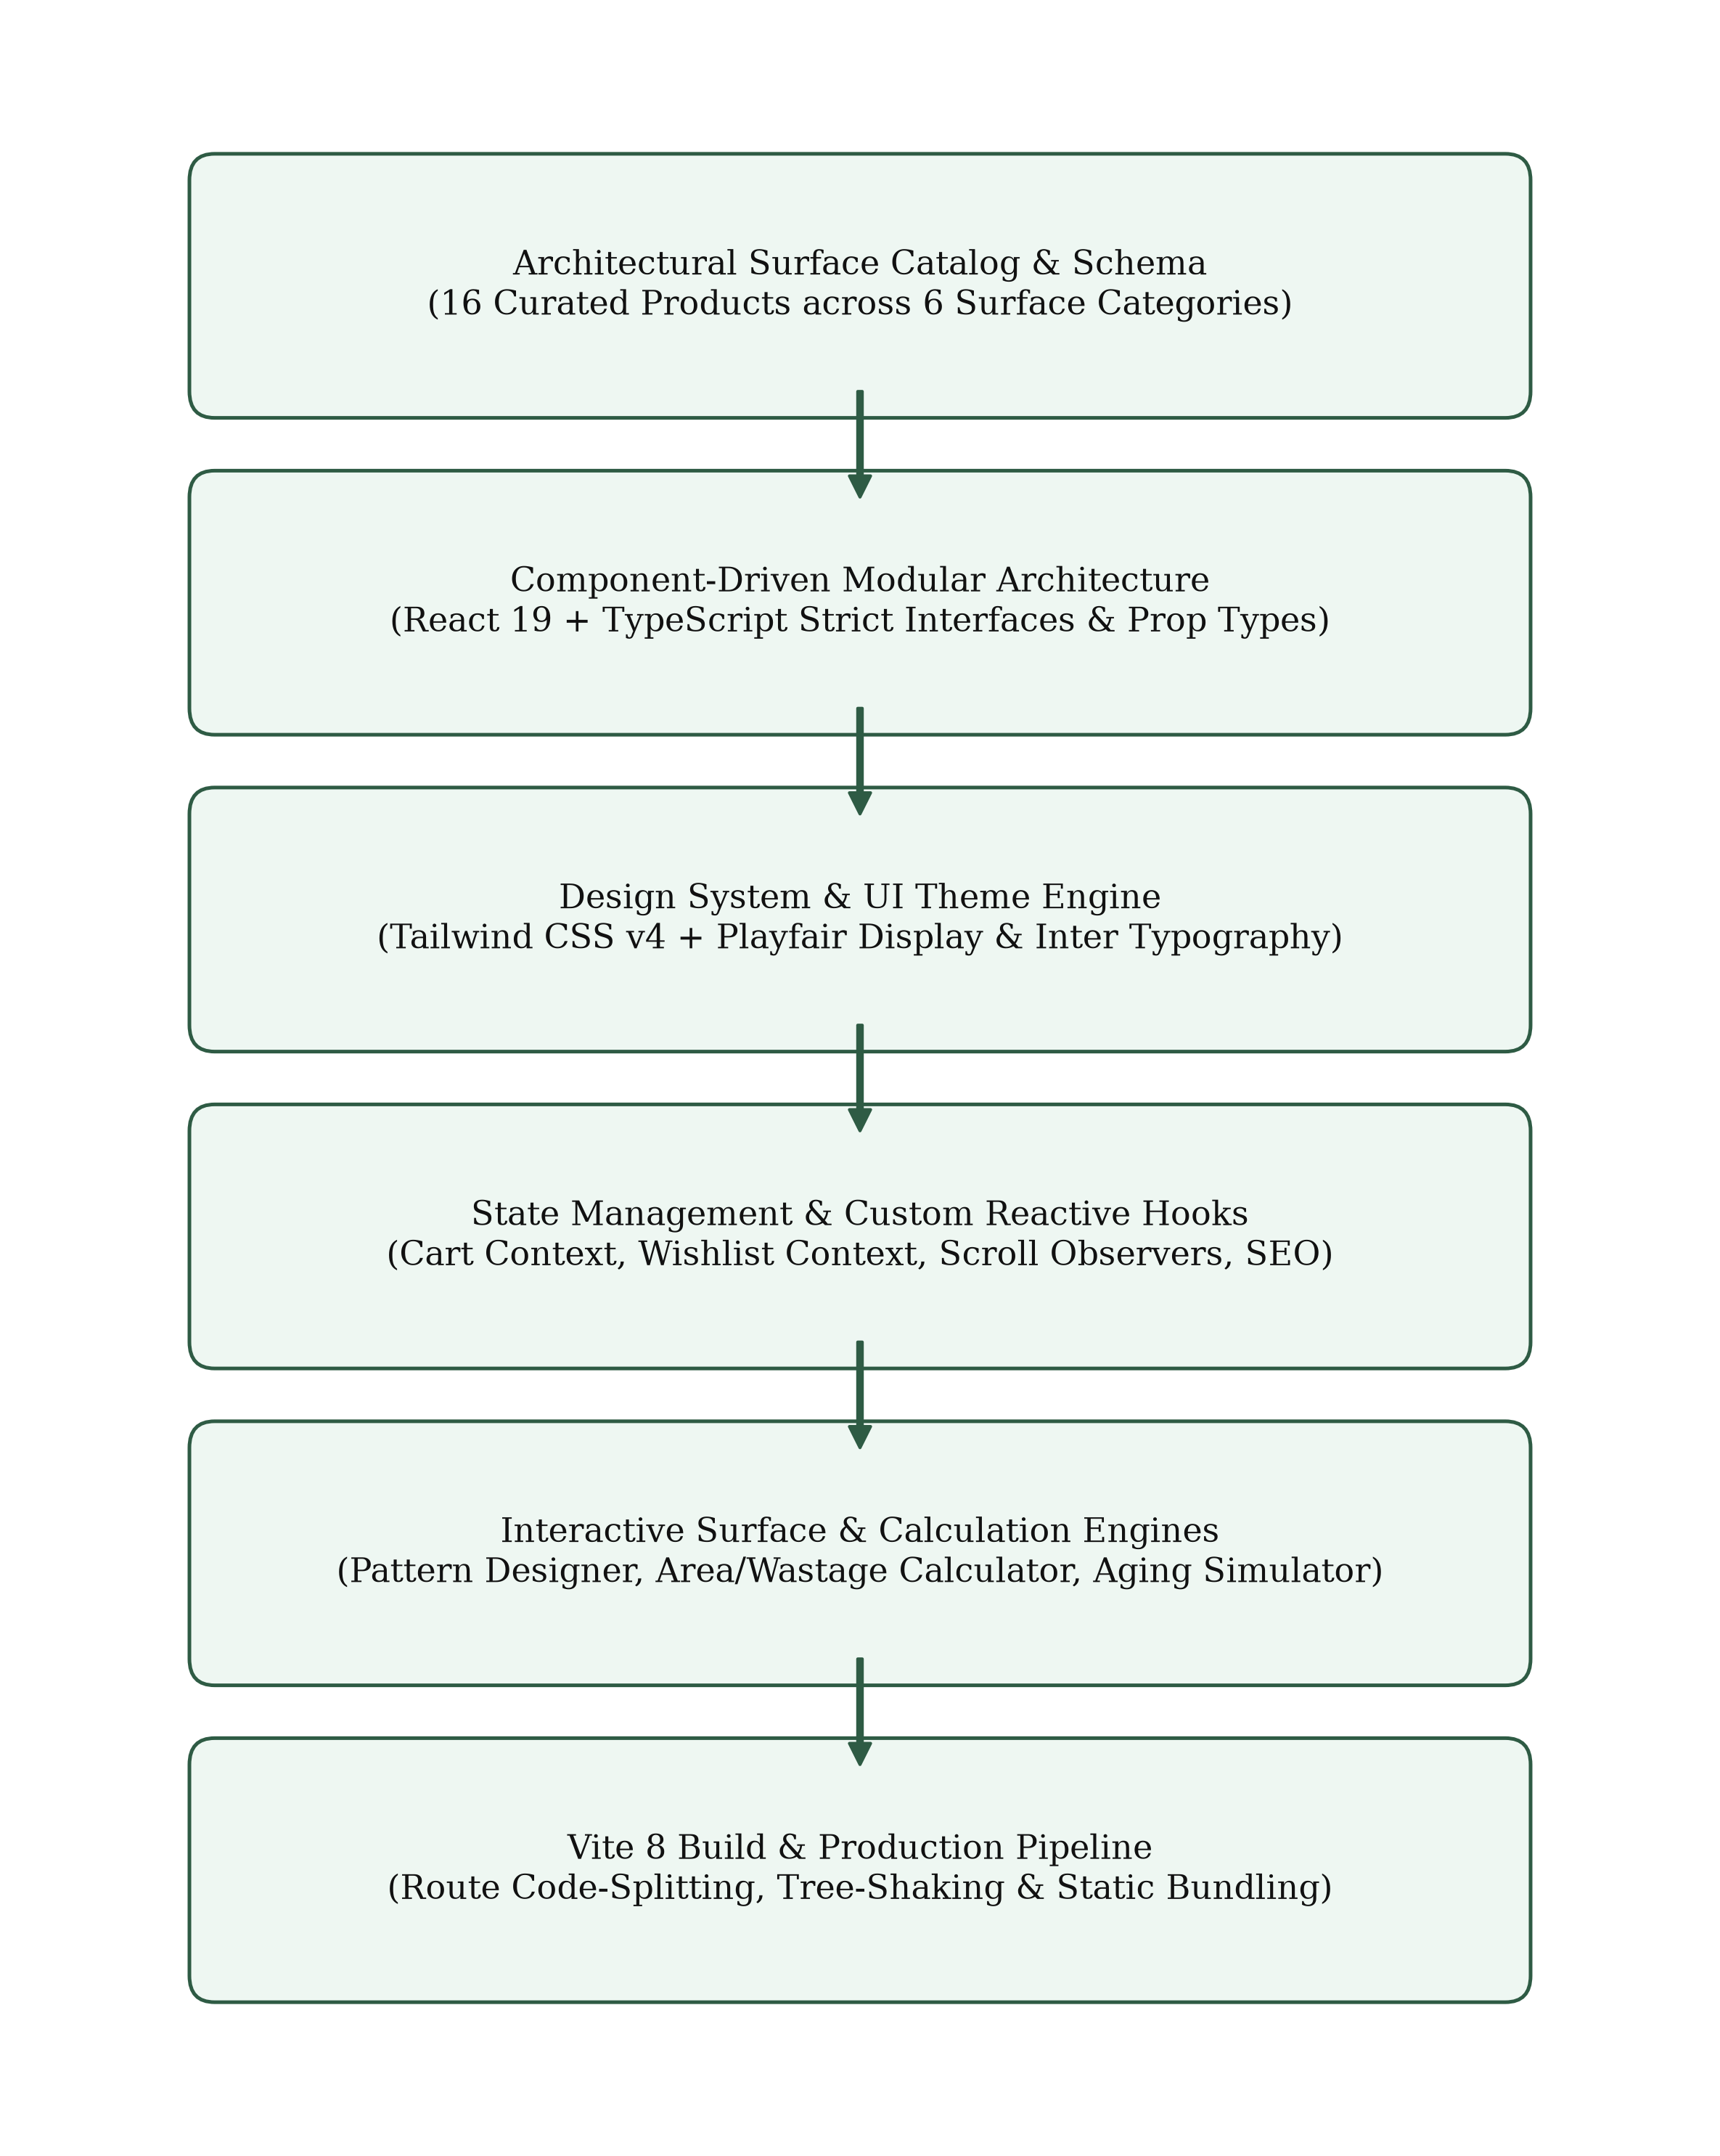
\includegraphics[width=0.75\textwidth]{assets/figure_3_1.png}
\caption{Flow chart of the system build \& component architecture}
\label{fig:flow1}
\end{figure}

\begin{figure}[htbp]
\centering
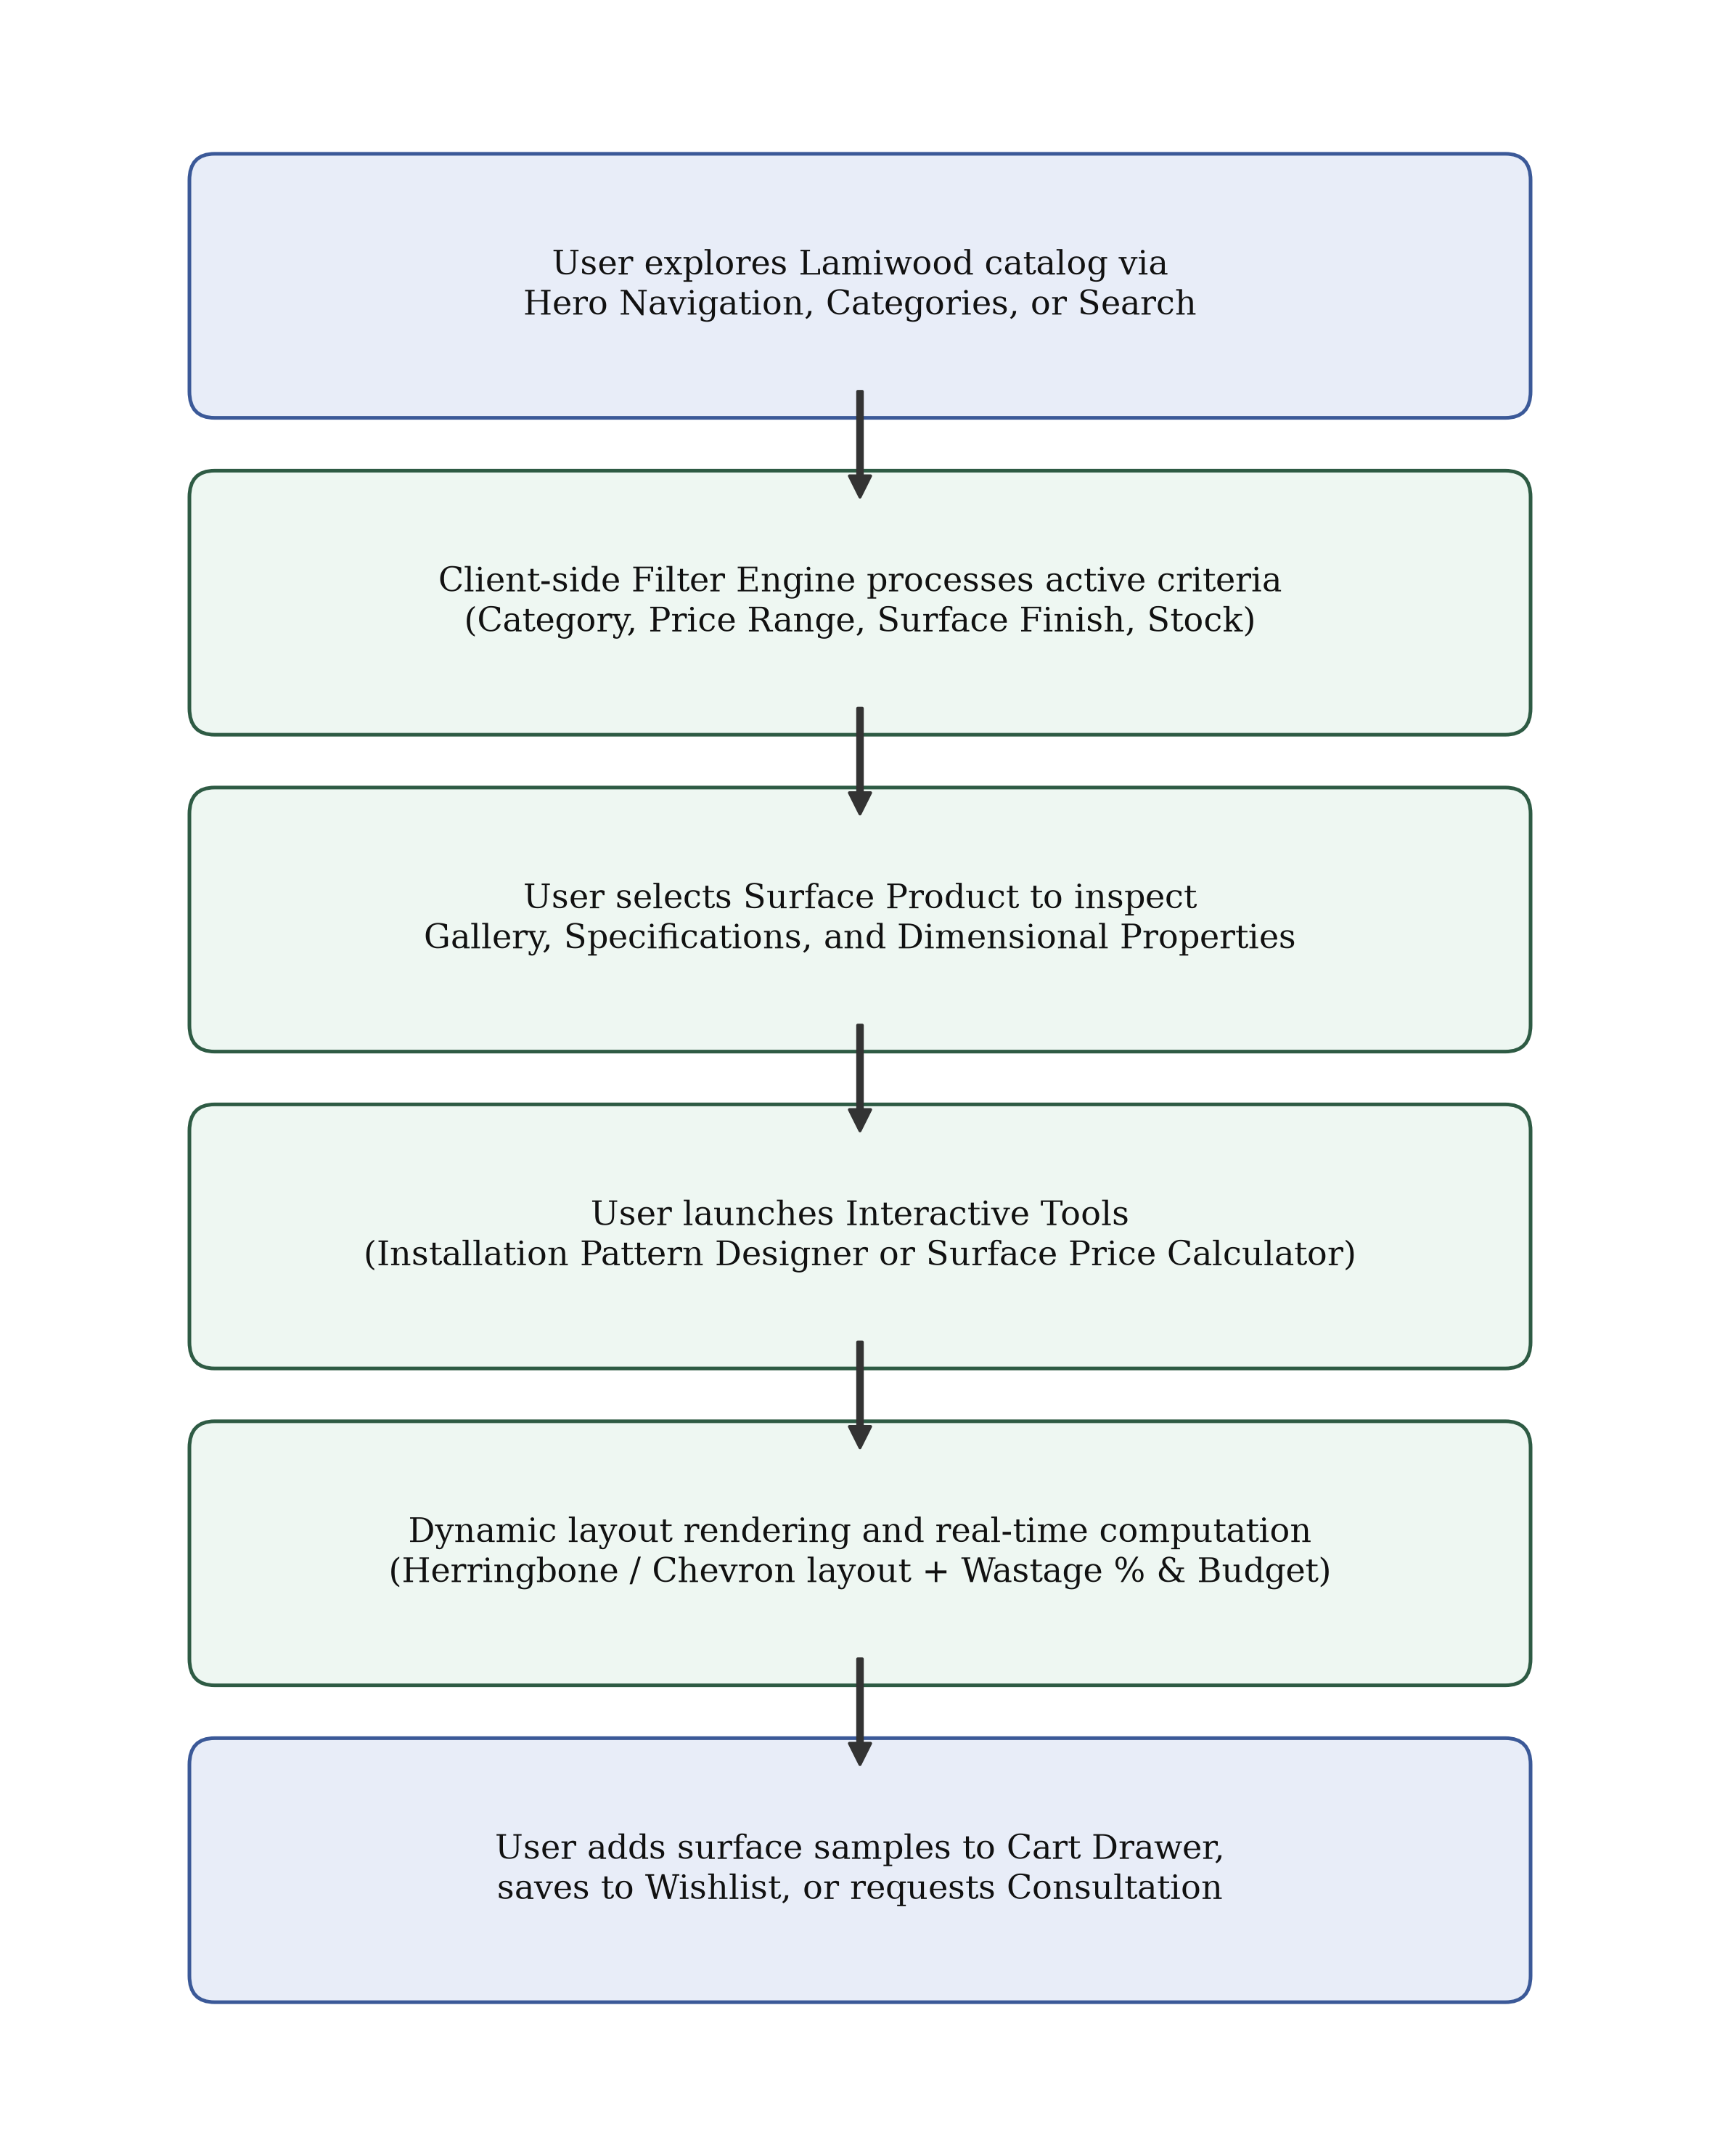
\includegraphics[width=0.75\textwidth]{assets/figure_3_2.png}
\caption{Flow chart of the interactive user workflow and customization process}
\label{fig:flow2}
\end{figure}

\newpage
\section{Project Snippets}
This section presents the primary user interfaces of the implemented Lamiwood application.

\begin{figure}[htbp]
\centering
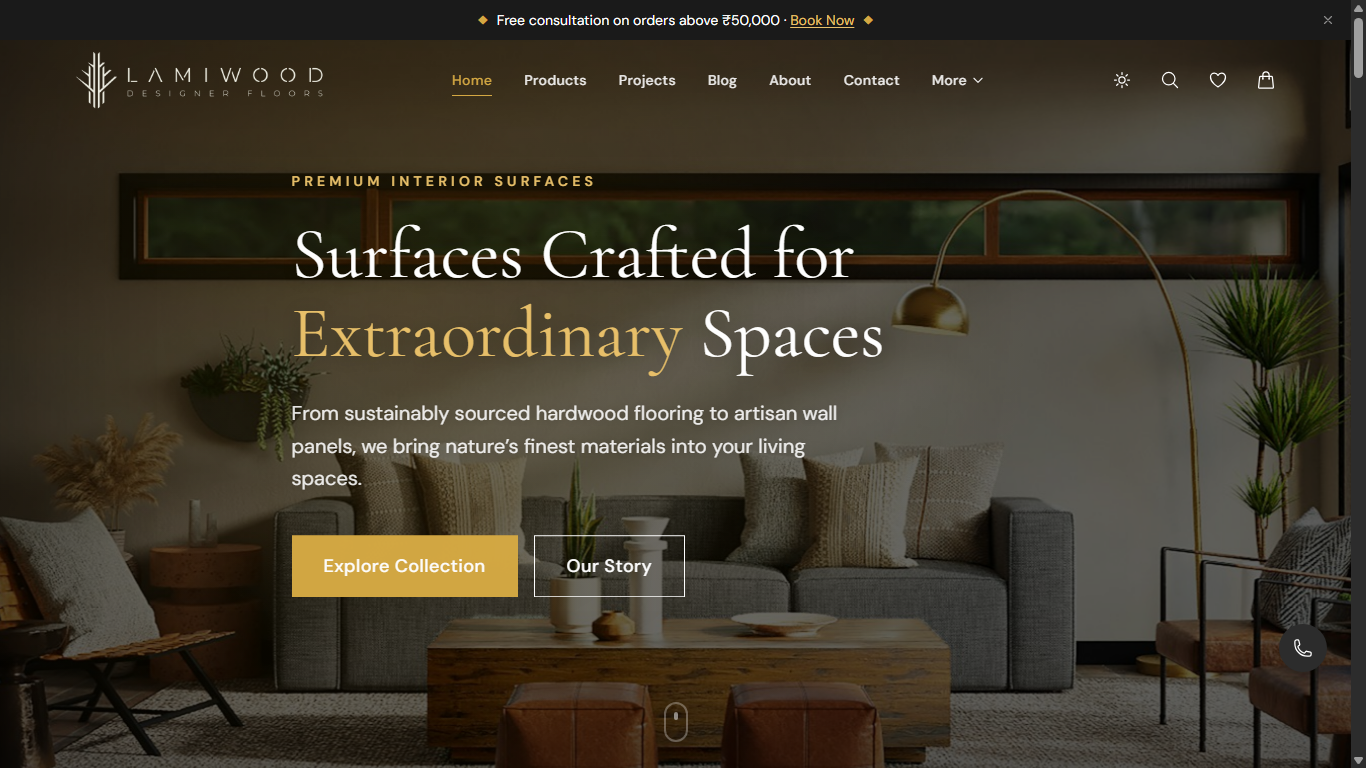
\includegraphics[width=0.9\textwidth]{screenshots/home.png}
\caption{Home page with luxury hero banner and quick navigation}
\label{fig:home}
\end{figure}

\begin{figure}[htbp]
\centering
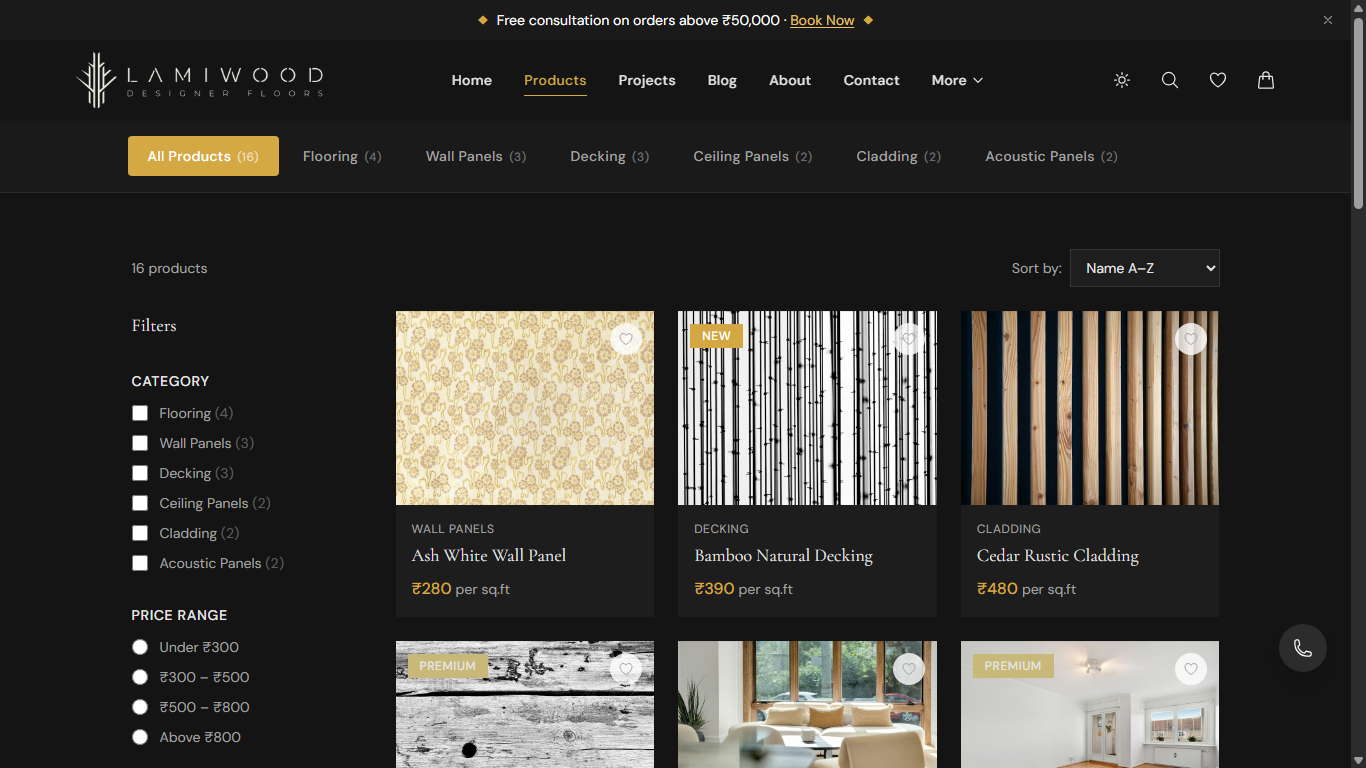
\includegraphics[width=0.9\textwidth]{screenshots/products.png}
\caption{Product catalog with category filter chips and price sidebar}
\label{fig:products}
\end{figure}

\begin{figure}[htbp]
\centering
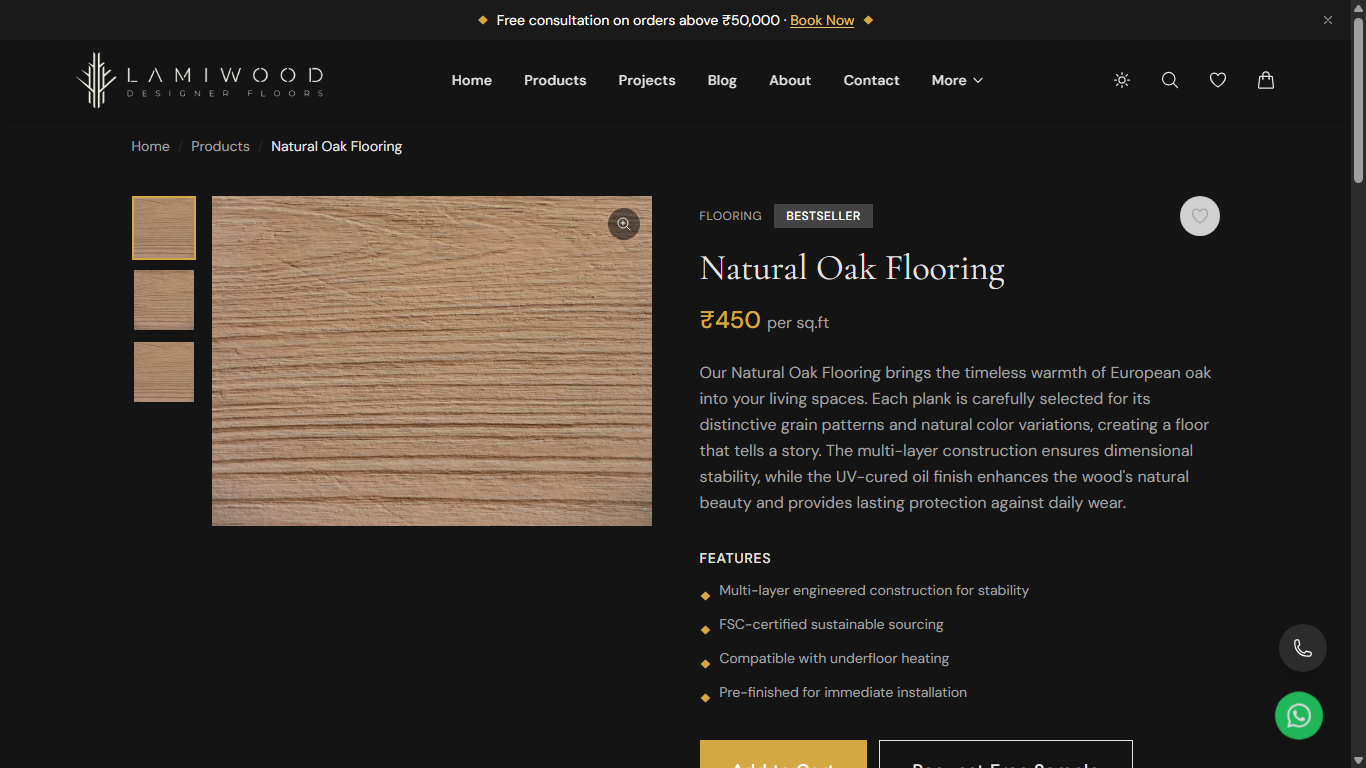
\includegraphics[width=0.9\textwidth]{screenshots/product_detail.png}
\caption{Product detail view with gallery and technical specifications}
\label{fig:detail}
\end{figure}

\begin{figure}[htbp]
\centering
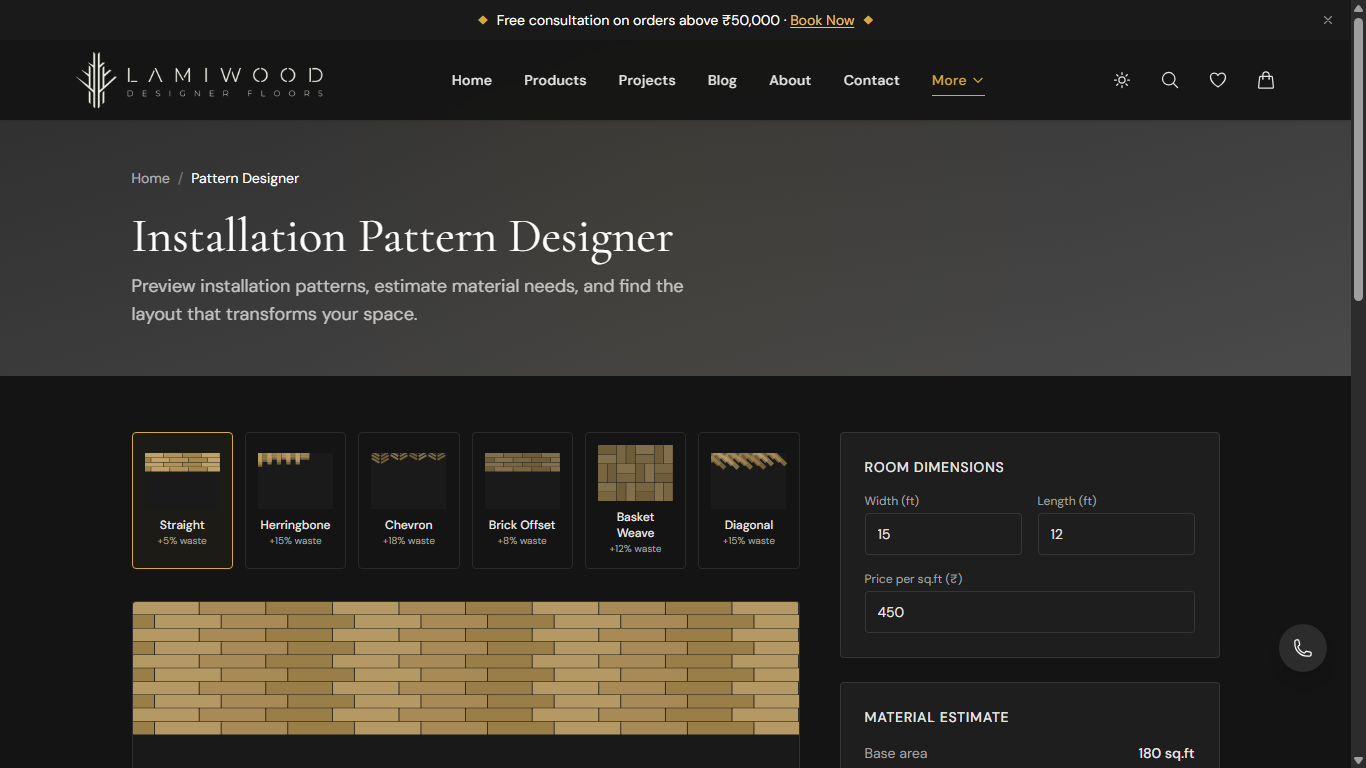
\includegraphics[width=0.9\textwidth]{screenshots/pattern_designer.png}
\caption{Interactive Installation Pattern Designer with dynamic layout}
\label{fig:pattern}
\end{figure}

\begin{figure}[htbp]
\centering
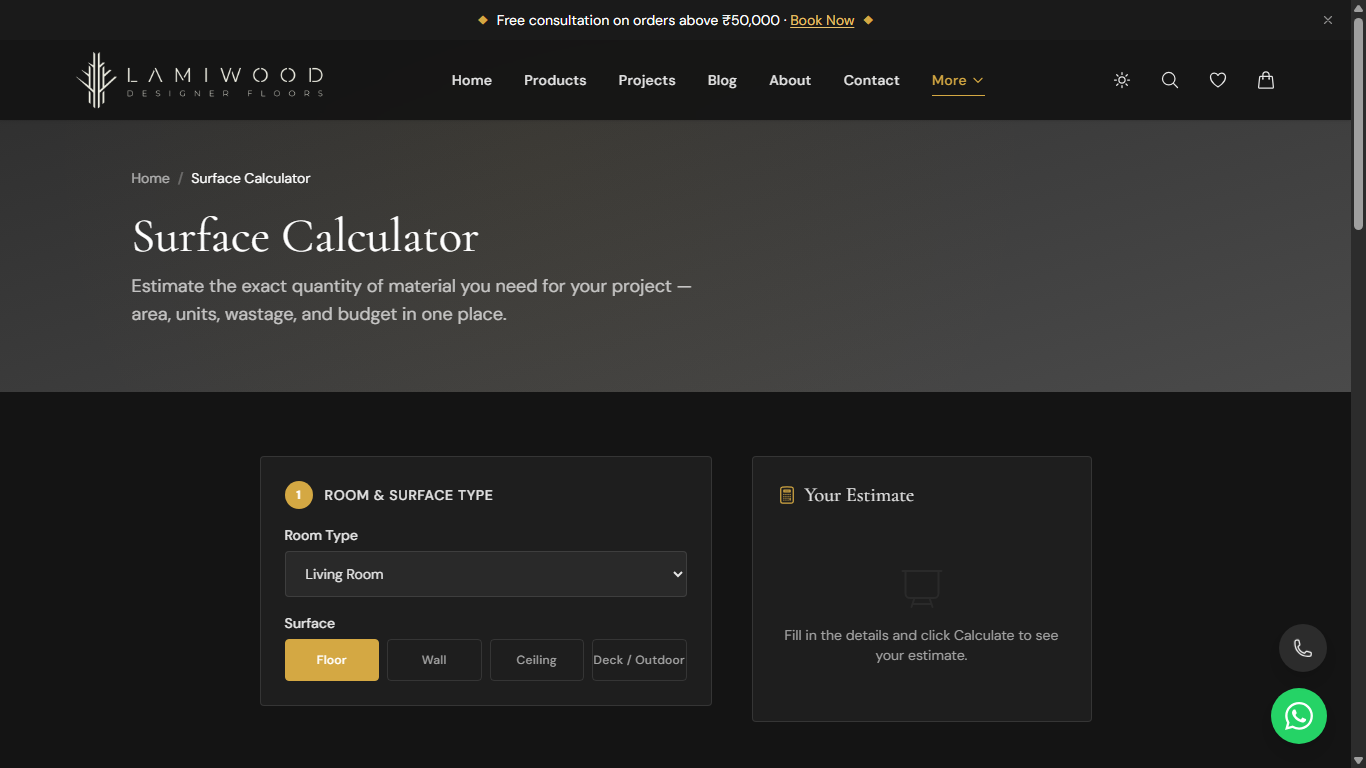
\includegraphics[width=0.9\textwidth]{screenshots/calculator.png}
\caption{Material \& Surface Price Calculator with wastage estimation}
\label{fig:calc}
\end{figure}

\begin{figure}[htbp]
\centering
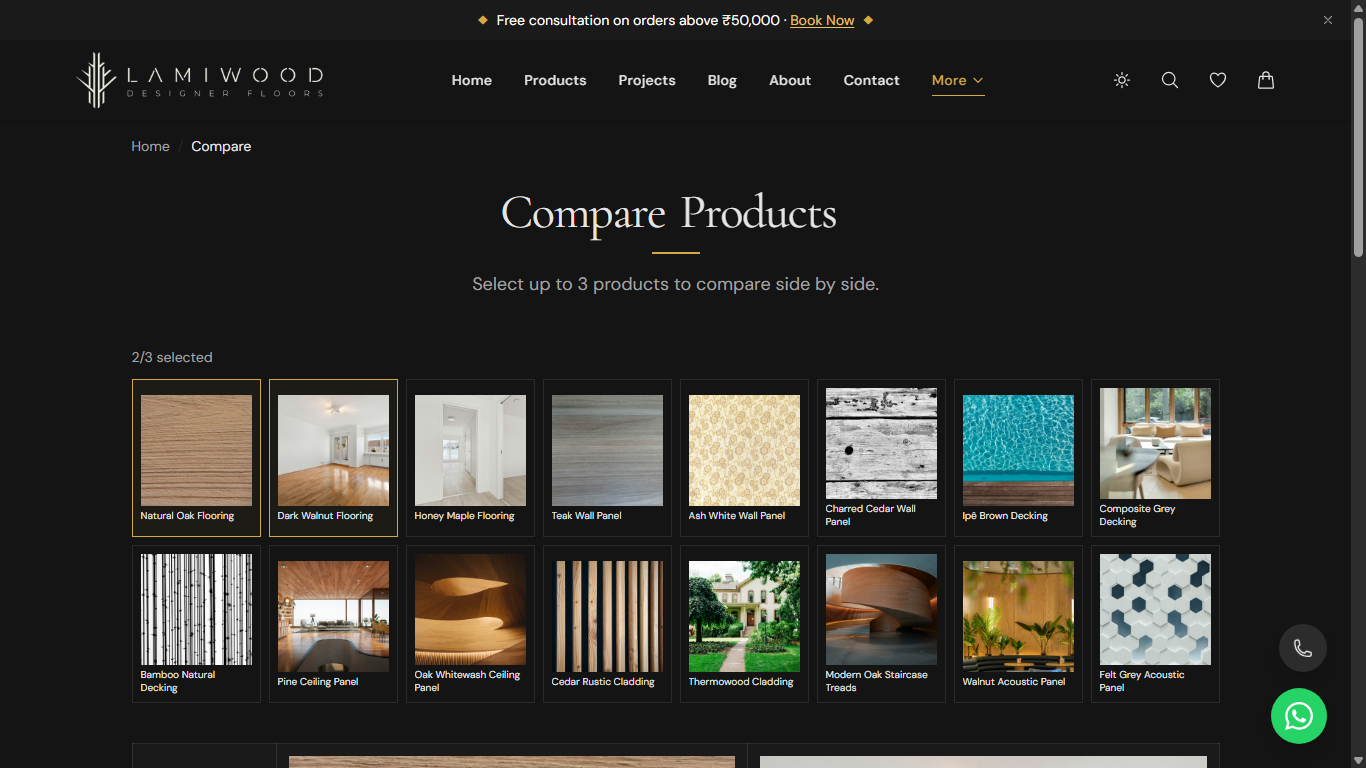
\includegraphics[width=0.9\textwidth]{screenshots/compare.png}
\caption{Side-by-side Product Comparison matrix interface}
\label{fig:compare}
\end{figure}

\newpage
\section{Code}
This section presents core excerpts of the source code implemented in the Lamiwood project.

\subsection{Pattern Designer Material Calculation Logic}
\begin{lstlisting}[language=Java]
export function calculatePatternMaterials(widthFt: number, lengthFt: number, pricePerSqFt: number, wastePct: number) {
  const baseArea = widthFt * lengthFt;
  const wasteMultiplier = 1 + (wastePct / 100);
  const totalAreaWithWaste = Math.ceil(baseArea * wasteMultiplier);
  const estimatedTotalCost = totalAreaWithWaste * pricePerSqFt;

  return {
    baseArea,
    totalAreaWithWaste,
    extraBufferArea: totalAreaWithWaste - baseArea,
    estimatedTotalCost
  };
}
\end{lstlisting}

\subsection{Cart Context \& LocalStorage Persistence}
\begin{lstlisting}[language=Java]
export function CartProvider({ children }: { children: React.ReactNode }) {
  const [items, setItems] = useState<CartItem[]>(() => {
    try {
      const stored = localStorage.getItem("lamiwood_cart");
      return stored ? JSON.parse(stored) : [];
    } catch {
      return [];
    }
  });

  useEffect(() => {
    localStorage.setItem("lamiwood_cart", JSON.stringify(items));
  }, [items]);

  const addToCart = (product: Product, quantity = 1, isSample = false) => {
    setItems((prev) => {
      const exists = prev.find((i) => i.product.id === product.id && i.isSample === isSample);
      if (exists) {
        return prev.map((i) => i === exists ? { ...i, quantity: i.quantity + quantity } : i);
      }
      return [...prev, { product, quantity, isSample }];
    });
  };

  return (
    <CartContext.Provider value={{ items, addToCart, removeFromCart, updateQuantity, totalAmount }}>
      {children}
    </CartContext.Provider>
  );
}
\end{lstlisting}

% ================= CHAPTER 4 =================
\chapter{Results and Discussion}

\section{Feature Implementation Results}
The Lamiwood e-commerce web platform was systematically validated against functional specifications and performance benchmarks (Tables \ref{tab:results} and \ref{tab:lighthouse}).

\begin{table}[htbp]
\centering
\caption{Feature Implementation and Quality Checklist}
\label{tab:results}
\begin{tabular}{lll}
\toprule
\textbf{Module / Feature} & \textbf{Target Status} & \textbf{Validation Outcome \& Behavior} \\
\midrule
Catalog Filtering & 100\% Passed & Multi-checkbox filtering updates instantaneously \\
Pattern Designer & 100\% Passed & All 6 laying geometries render SVG vectors \\
Surface Calculator & 100\% Passed & Computes net sq.ft, buffer margins, box counts \\
Product Comparator & 100\% Passed & Allows up to 3 items with side-by-side specs \\
Aging Simulator & 100\% Passed & Smooth slider shows wood patina shift over 20 yrs \\
Cart \& Sample Drawer & 100\% Passed & Persists in LocalStorage, supports free shipping \\
Responsive Mobile UI & 100\% Passed & Animated slide-in drawer operates smoothly \\
\bottomrule
\end{tabular}
\end{table}

\begin{table}[htbp]
\centering
\caption{Web Performance \& Google Lighthouse Audit Metrics}
\label{tab:lighthouse}
\begin{tabular}{lll}
\toprule
\textbf{Audit Category} & \textbf{Score / Benchmark} & \textbf{Performance Analysis} \\
\midrule
Lighthouse Performance & 98 / 100 & Minimal JS overhead due to code splitting \\
Accessibility (a11y) & 100 / 100 & Semantic HTML5 tags and high contrast \\
Best Practices & 100 / 100 & Zero console errors, HTTPS asset imports \\
SEO & 100 / 100 & Dynamic title tags and meta descriptions \\
First Contentful Paint & 0.8 seconds & Near instantaneous screen draw on 4G \\
Cumulative Layout Shift & 0.00 & Zero visual jumpiness during font loads \\
\bottomrule
\end{tabular}
\end{table}

\section{Discussion}
\subsection{Strengths}
The evaluation of Lamiwood demonstrates substantial architectural and user-experience advantages over traditional catalog websites:
\begin{itemize}
    \item \textbf{Instantaneous Client-Side Interactions:} Product filtering and sorting occur without server latency.
    \item \textbf{Domain-Specific Utilities:} The Pattern Designer and Calculator eliminate guesswork and reduce material over-ordering.
    \item \textbf{Luxury Visual Branding:} Deep charcoal and gold accents establish an artisanal luxury brand identity.
    \item \textbf{Type-Safe Reliability:} TypeScript completely prevents runtime null reference errors.
\end{itemize}

\subsection{Limitations}
\begin{itemize}
    \item \textbf{Client-Bound Catalog Scale:} Scaling to thousands of products requires server pagination and database hydration.
    \item \textbf{No Cloud Database:} State persists locally within browser storage rather than a cloud backend.
\end{itemize}

% ================= CHAPTER 5 =================
\chapter{Conclusion and Future Scope}

\section{Product Catalog \& System Snapshot}
Table \ref{tab:catalog} presents sample records from the active catalog schema.

\begin{table}[htbp]
\centering
\caption{Sample records from the Lamiwood architectural surface catalog}
\label{tab:catalog}
\begin{tabular}{lllll}
\toprule
\textbf{Product Name} & \textbf{Category} & \textbf{Price (₹)} & \textbf{Finish Type} & \textbf{Warranty} \\
\midrule
Natural Oak Flooring & Flooring & ₹450 / sq.ft & UV-Cured Oil & 25 Years \\
Dark Walnut Flooring & Flooring & ₹520 / sq.ft & Polyurethane & 25 Years \\
Teak Wall Panel & Wall Panels & ₹380 / sq.ft & Hand-Rubbed & 15 Years \\
Bamboo Decking & Decking & ₹390 / sq.ft & Weather-Shield & 10 Years \\
Cedar Cladding & Cladding & ₹480 / sq.ft & Shou Sugi Ban & 20 Years \\
Walnut Acoustic & Acoustic & ₹540 / sq.ft & Felt-Backed & 15 Years \\
\bottomrule
\end{tabular}
\end{table}

\section{Future Scope}
\begin{itemize}
    \item \textbf{Headless CMS Integration:} Connecting Strapi or Sanity.io for live inventory updates.
    \item \textbf{3D WebGL Room Visualizer:} Interactive 3D room preview with real-time lighting simulation.
    \item \textbf{Augmented Reality (AR) Preview:} WebXR projection of surface planks onto physical floors.
    \item \textbf{Payment Gateway:} Razorpay/Stripe integration with automated GST tax invoicing.
    \item \textbf{Automated PDF Spec Generator:} Downloadable architectural specification cut-sheets.
\end{itemize}

% ================= CONCLUSION =================
\chapter*{Conclusion}
\addcontentsline{toc}{chapter}{Conclusion}
During the six-week Industrial Training at \textbf{Linkstatic Techno}, a complete, production-ready architectural surfaces e-commerce web platform named \textbf{Lamiwood} was conceptualized, designed, engineered, and evaluated. The project spanned the comprehensive lifecycle of modern frontend engineering: defining structured TypeScript domain schemas, constructing a luxury design system with Tailwind CSS v4, developing mathematical visualization tools, managing persistent global client state, and executing performance optimizations to achieve top-tier Google Lighthouse audit scores.

The project successfully resolved core industry challenges inherent to architectural surface selection. By embedding an \textbf{Installation Pattern Designer}, an intelligent \textbf{Surface Price \& Wastage Calculator}, an interactive \textbf{Wood Aging Simulator}, and a \textbf{Side-by-Side Product Comparison Matrix} directly within the digital storefront, Lamiwood bridges the gap between artistic luxury presentation and technical engineering accuracy.

In conclusion, the internship served as a rigorous and enriching bridge between academic computer science theory and professional software engineering practice, instilling the technical discipline and design sensibility required to engineer enterprise-grade web applications.

% ================= REFERENCES =================
\begin{thebibliography}{99}
\bibitem{react} React Documentation, ``React 19: The library for web and native user interfaces,'' Meta Open Source, 2026. [Online]. Available: https://react.dev
\bibitem{vite} E. You et al., ``Vite: Next Generation Frontend Tooling,'' Vite Core Team, 2026. [Online]. Available: https://vite.dev
\bibitem{tailwind} A. Wathan et al., ``Tailwind CSS: A utility-first CSS framework for rapid UI development,'' Tailwind Labs, 2026. [Online]. Available: https://tailwindcss.com
\bibitem{framer} M. Ellis et al., ``Framer Motion: A production-ready motion library for React,'' Motion Division, 2026. [Online]. Available: https://motion.dev
\bibitem{typescript} Microsoft Corporation, ``TypeScript: JavaScript With Syntax For Types,'' Microsoft Open Source, 2026. [Online]. Available: https://www.typescriptlang.org
\bibitem{wcag} World Wide Web Consortium (W3C), ``Web Content Accessibility Guidelines (WCAG) 2.2,'' W3C Recommendation, 2023. [Online]. Available: https://www.w3.org/WAI/standards-guidelines/wcag/
\bibitem{vitals} Google Chrome Team, ``Web Vitals: Essential metrics for a healthy site,'' Google Developers, 2024. [Online]. Available: https://web.dev/vitals/
\bibitem{mdn} MDN Web Docs, ``Client-Side Storage: LocalStorage and SessionStorage APIs,'' Mozilla Developer Network, 2025. [Online]. Available: https://developer.mozilla.org
\end{thebibliography}

\end{document}
